\subsection{Comparisons with the original lattice implementations}
\label{sec:state-comparisons}
We define squared fidelity $F=|\langle\psi|\phi\rangle|^2$ for normalized
vectors, infidelity $1-F$, and matrix error
$\|M\|_F=(\Tr M^\dagger M)^{1/2}$. The most useful energy ratio uses
\emph{excitation gaps}, since ratios of extensive total energies are
insensitive to the excitation:
\begin{equation}
 E_I=-2\csc\frac\pi{2N},\quad E_\sigma=-2\cot\frac\pi{2N},\quad
 E_\eps=E_I+8\sin\frac\pi{2N},\quad
 R_E=\frac{E_\eps-E_I}{E_\sigma-E_I}=8\cos^2\frac\pi{4N}.
 \label{eq:gaps}
\end{equation}
The continuum limit is $R_E\to8$, from dimensions $1$ and $1/8$.
With the velocity $v=2$ of Eq.~\eqref{eq:Hising}, the relation
$E_a-E_I\sim(2\pi v/N)(h_a+\bar h_a)$ identifies
the $\eps$ and $\sigma$ dimensions as $1$ and $1/8$, respectively.

\begin{table}[htbp]\centering\small
\begin{tabular}{rrlrrrr}\toprule
$N$ & $D_{\rm bond}$ & State & Infidelity & $|E_{\rm puMPS}-E_{\rm CB}|$ & $\eta_{\rm puMPS}$ & $\|\Delta\rho_4\|_F$\\\midrule
10 & 8 & $I$ & $1.65\!\times\!10^{-9}$ & $1.95\!\times\!10^{-8}$ & $4.88\!\times\!10^{-4}$ & $1.91\!\times\!10^{-6}$ \\
10 & 8 & $\sigma$ & $3.97\!\times\!10^{-8}$ & $5.18\!\times\!10^{-7}$ & 0.0026512 & $6.23\!\times\!10^{-6}$ \\
10 & 8 & $\varepsilon$ & $1.64\!\times\!10^{-7}$ & $1.93\!\times\!10^{-6}$ & 0.0048855 & $2.46\!\times\!10^{-5}$ \\
16 & 14 & $I$ & $2.62\!\times\!10^{-10}$ & $2.81\!\times\!10^{-9}$ & $1.81\!\times\!10^{-4}$ & $2.33\!\times\!10^{-6}$ \\
16 & 14 & $\sigma$ & $6.34\!\times\!10^{-8}$ & $7.61\!\times\!10^{-7}$ & 0.0031009 & $2.89\!\times\!10^{-6}$ \\
16 & 14 & $\varepsilon$ & $3.99\!\times\!10^{-7}$ & $4.30\!\times\!10^{-6}$ & 0.007004 & $1.46\!\times\!10^{-5}$ \\
\bottomrule\end{tabular}

\caption{Fresh full-vector comparisons with archived puMPS checkpoints.
$D_{\rm bond}$ is the MPS bond dimension, distinct from relative entropy.
The seed is $1234+N$ in the archived optimization. $I$ and $\eps$ use pure
CB vectors, while $\sigma$ uses Eq.~\eqref{eq:projection}. All vectors
are normalized, all energies use Eq.~\eqref{eq:Hising}, and the interval
matrix comparison has $\ell=4$. Every reported infidelity is below
$4.0\times10^{-7}$. No puMPS reoptimization is claimed.}
\label{tab:pumps}
\end{table}

For the Laughlin comparison, the new code places site zero in the least
significant bit, whereas the original dense constructor uses the most
significant bit. We reverse bit order before comparing the vectors;
the comparison then tests branches, phases and normalization in the
same physical basis.
Fresh Laughlin-vector comparisons at $N=8,10,12$, for all three boson
states and $W=10^8$, give $|1-F|\leq1.8\times10^{-15}$ and maximum
phase-aligned amplitude error $4.1\times10^{-15}$.
For the Haldane--Shastry convention in Eq.~\eqref{eq:HHS}, the measured
gap ratios $(E_{3s,s}-E_{00})/(E_{ss}-E_{00})$ are
$4,4.2,13/3$ at $N=8,10,12$, approaching the CFT value five.
At finite $W$, excited-state eigen residuals are below $6.3\times10^{-9}$.

Ising blocks were tested against independent exact diagonalization through
$N=12$, and against exact-fermion interval matrices for every requested
$N\leq24$. The full $I$ and $\eps$ CB vectors were evaluated even at
$N=24$. Exact-fermion production for $\sigma$ is cross-checked against the
projected vectors through $N=16$. Numerical CSVs retain every test value.
For the covariance calculation, the code also enforces
$\max_{r,s}|(G^2+\id)_{rs}|<2\times10^{-12}$.
The baseline 150 boson values agree with the original 150 values
within $1.16\times10^{-11}$. Ising differences from the available puMPS
grid are at most $4.15\times10^{-7}$ across $\ell=2,\ldots,6$.
Historical $N=22$ puMPS states were excluded because their mutual overlaps
failed a quality criterion. Our $N=22$ data are newly generated exact-chain
data, explicitly marked as such; we have not repaired or silently
reinstated those puMPS checkpoints.

\subsubsection{Numerical evidence for the Ising reference}
\label{sec:method-quality-checks}
We choose the exact finite-chain Ising states as the primary input to the
relative-entropy study because their preparation error is independently
controlled. The conformal-block vectors for $I,\eps$ and the projected
vector for $\sigma$ verify the state identification; the exact fermion
covariances provide the interval matrices used in the fits.
The decision is supported by the following comparison with the original
periodic uniform matrix product states (puMPS).

\begin{table}[htbp]\centering\small
\begin{tabular}{lrrrl}\toprule
State & $\eta_{\rm puMPS}$ & $\eta_{\rm new}$ & $1-F$ & New vector\\\midrule
$I$ & $1.81\times10^{-4}$ & $1.24\times10^{-12}$ & $2.62\times10^{-10}$ & Vacuum block \\
$\sigma$ & $3.10\times10^{-3}$ & $2.70\times10^{-12}$ & $6.34\times10^{-8}$ & Block-seeded Lanczos \\
$\varepsilon$ & $7.00\times10^{-3}$ & $3.35\times10^{-12}$ & $3.99\times10^{-7}$ & Endpoint block \\
\bottomrule\end{tabular}

\caption{Accuracy comparison at $N=16$ against the archived puMPS
checkpoint of bond dimension $D_{\rm bond}=14$, optimization seed $1250$.
All vectors are normalized and use Eq.~\eqref{eq:Hising} with both
couplings equal to one and periodic spin boundaries.
The residual $\eta$ is defined by Eq.~\eqref{eq:eigenresidual};
$1-F=1-|\langle\psi_{\rm new}|\psi_{\rm puMPS}\rangle|^2$ is the
infidelity. The new $\sigma$ vector uses block-seeded Lanczos, with
requested solver tolerance $2\times10^{-12}$, rather than a pure
conformal-block formula. Entries are from the original whole-vector
validation CSVs; no puMPS reoptimization is performed.}
\label{tab:methodquality}
\end{table}

\begin{enumerate}
\item \textbf{The tested finite-chain eigenstate errors are smaller.}
Table~\ref{tab:methodquality} shows residuals near $10^{-12}$ for the
new vectors, compared with $10^{-4}$--$10^{-2}$ for the archived puMPS
vectors. Their energy ordering and symmetries also match the exact
solution, so the small residuals do not merely identify unrelated
eigenstates. The full $N=10,16$ overlap and energy comparisons are in
Table~\ref{tab:pumps}.
\item \textbf{The reduced states have an independent reference.}
For $I,\eps$, direct partial traces of the conformal-block vectors agree
with the exact fermion interval matrices to a maximum Frobenius error
of $1.55\times10^{-13}$ over the original sizes
$N=16,18,20,22,24$ and $\ell=2,\ldots,6$.
For $\sigma$, the projected vectors were independently compared with
the exact fermion reduced states through $N=16$.
\item \textbf{The same construction covers the full requested size grid.}
It supplies exact-chain data at $N=22$, where the archived puMPS
checkpoint did not pass the earlier overlap-quality criterion.
The new calculation has its own provenance and does not rehabilitate
that checkpoint.
\end{enumerate}

The scope of this preference is finite-chain accuracy for this integrable
Hamiltonian. The archived puMPS vectors are already close in overlap,
with infidelity below $4\times10^{-7}$ in all tested comparisons.
Larger bond dimensions or improved optimization could reduce their
remaining errors; the tests do not establish that conformal blocks are
universally superior to converged puMPS. The $\sigma$ accuracy relies on
Hamiltonian projection and the exact fermion solution. Finally, exact
lattice eigenstates still have finite-size and short-interval lattice
corrections. Improving their preparation therefore does not, by itself,
remove the discrepancies with continuum coefficients at $\ell=2,3,4$.


\begin{figure}[htbp]\centering
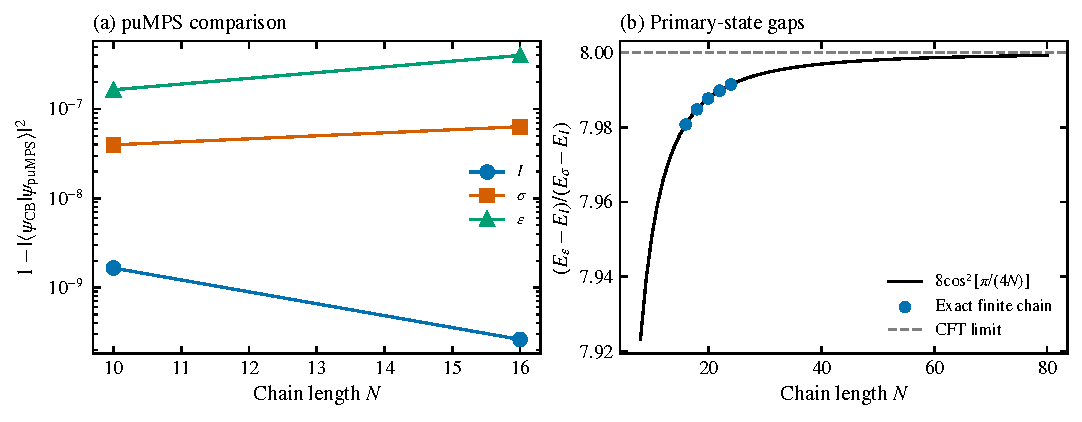
\includegraphics[width=\linewidth]{../figs/state_validation.pdf}
\caption{State validation at critical coupling and periodic spin boundaries.
(a) Squared-overlap infidelities against archived puMPS at
$(N,D_{\rm bond})=(10,8),(16,14)$, seeds $1244,1250$; $\sigma$ uses the
CB-seeded projection with solver tolerance $2\times10^{-12}$.
(b) Exact finite-chain gap ratios at $N=16,18,20,22,24$ and
Eq.~\eqref{eq:gaps}; the dashed line is the continuum value eight.
No interval length or mixture probability enters these whole-state tests.}
\label{fig:validation}
\end{figure}
